\begin{figure*}%
	\centering%
	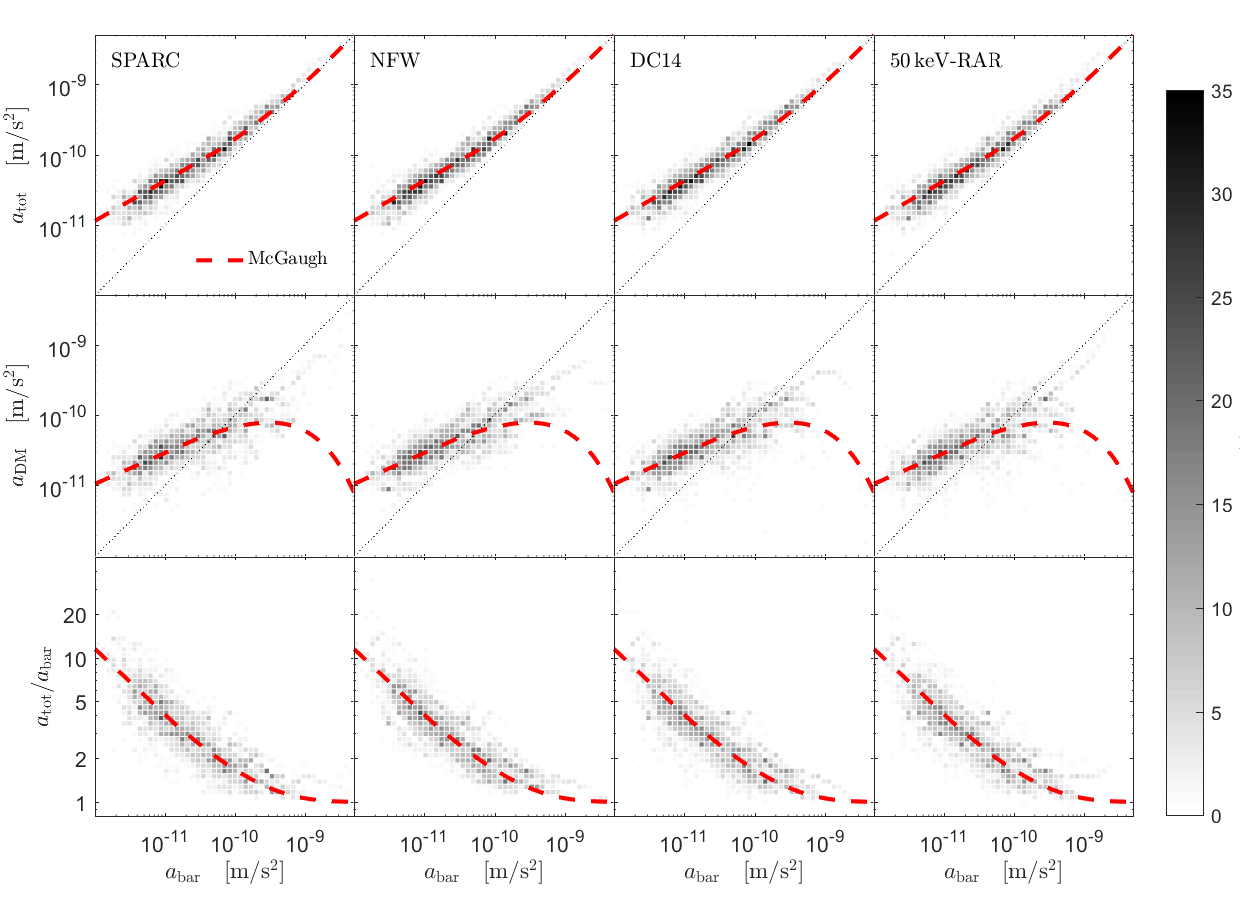
\includegraphics[width=\hsize]{\ROOTPATH/fig.png}
	\caption{Radial acceleration correlations from SPARC data (first row), NFW (second row), DC14 (third) and RAR (forth row). The correlation is presented in three different ways: (top panels) original correlation with focus on the total acceleration $a_{\rm tot}$, (middle panels) correlation with focus on the dark component $\SYMaDM$ and (bottom panels) the mass discrepancy acceleration relation with focus on the ratio $a_{\rm tot}/a_{\rm bar}$. The baryonic centripetal acceleration $a_{\rm bar}$ is inferred from luminosity observables while the total acceleration is inferred from velocity fields. Both measurements are independent. For SPARC data the inferred DM acceleration is given by $\SYMaDM = \SYMaobs - \SYMabar$. In the case of RAR, NFW and DC14 the total acceleration is composed of the predicted dark and the inferred baryonic components. Each plot is divided in 50x50 equal bins showing clearly a non-linear correlation. Note, that the top panels emphasize mainly the dark matter dominated region for accelerations below the particular value $\SYMafrak \approx 1.20 \times 10^{-10} \mathrm{m/s^2}$. Above that acceleration the information about dark matter is hidden due to the baryon dominance, what becomes unveiled in the middle panels. Qualitatively, all considered models (RAR,NFW,DC14) are able to reproduce the radial acceleration correlation, independent of the representations.}%
	\label{fig:acceleration:grid}%
\end{figure*}